\documentclass[border=3pt,tikz]{standalone}
\usepackage{amsmath}
\usetikzlibrary{calc}
\usetikzlibrary{arrows.meta} % for arrow size
\begin{document}

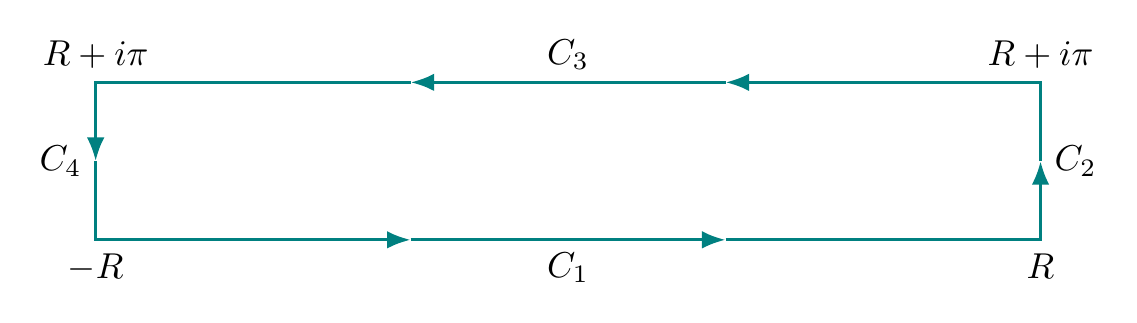
\begin{tikzpicture}[scale=2]
    \usetikzlibrary {arrows.meta}
    \usetikzlibrary {calc}
    
    \draw[teal, very thick, -{Latex[length = 3mm, inset=1.5]}] (-3, 0.5)
      -- (-3, 0) node[black, below, scale=1.3] {$-R$}
      -- (-1, 0);
    
    \node[below, scale=1.3] {$C_1$};
    \draw[teal, very thick,  -{Latex[length =3mm]}] (-1, 0) -- (1, 0);
      
    \draw[teal, very thick,  -{Latex[length =3mm]}] (1,0)
      -- (3, 0) node [black, below, scale=1.3] {$R$}
      -- (3, 0.5) node [black, right, scale=1.3] {$C_2$};
    \draw[teal, very thick,  -{Latex[length =3mm]}] (3, 0.5) 
      -- (3, 1) node [black, above, scale=1.3] {$R+i\pi$}
      -- (1, 1);
    
    \node[black, above, scale=1.3] at (0, 1) {$C_3$};
    \draw[teal, very thick, -{Latex[length =3mm]}] (1, 1) -- (-1, 1);
    \draw[teal, very thick, -{Latex[length =3mm]}] (-1, 1) 
      -- (-3, 1) node[black, above, scale=1.3] {$R+i\pi$}
      -- (-3, 0.5) node[black, left, scale=1.3] {$C_4$};
    
    \end{tikzpicture}
    
    
\end{document}